\documentclass[conference]{IEEEtran}

\usepackage[spanish]{babel}
\usepackage{amsmath,amssymb,amsfonts,amsthm}
\usepackage{graphicx}
%\usepackage{bbm}
\usepackage[utf8]{inputenc} % Caracteres en Español (Acentos, ñs)
\usepackage{url} % ACENTOS
\usepackage{hyperref} % Referencias
\usepackage{subfig}
\usepackage{lipsum}
\usepackage{balance}
\usepackage{colortbl}
\usepackage{xcolor}
\usepackage{array}
\usepackage{multirow} %Paquete para la doble row

%%%%%%%%%%%%%%%%%%%%%%%%%%%%%%%%%%%%%%%%%%%%%
% PARCHE PARA ELIMINAR LA FECHA DEL DOCUMENTO
% 
\usepackage{etoolbox}
\makeatletter
% \frontmatter@RRAP@format is responsible for the parentheses
\patchcmd{\frontmatter@RRAP@format}{(}{}{}{}
\patchcmd{\frontmatter@RRAP@format}{)}{}{}{}
%\renewcommand\Dated@name{}
\makeatother	
% FIN DEL PARCHE
% 
%%%%%%%%%%%%%%%%%%%%%%%%%%%%%%%%%%%%%%%%%%%%%

%%%%%%%%%%%%%%%%%%%%%%%%%%%%%%%%%%%%%%%%%%%%%
% PARCHE PARA PERMIRIR UTILIZAR BIBLATEX EN ESTA PANTLLA
%\PassOptionsToPackage{square,numbers}{natbib}
%\RequirePackage{natbib}  
%%%%%%%%%%%%%%%%%%%%%%%%%%%%%%%%%%%%%%%%%%%%%

\usepackage[backend=bibtex,sorting=none]{biblatex}
% Estas lineas permiten romper los hipervinculos muy largos !!!!
\setcounter{biburllcpenalty}{7000}
\setcounter{biburlucpenalty}{8000}
\addbibresource{references.bib}

% Actualiza en automático la fecha de las citas de internet a la fecha de la compilación del documento
\usepackage{datetime}
\newdateformat{specialdate}{\twodigit{\THEDAY}-\twodigit{\THEMONTH}-\THEYEAR}
\date{\specialdate\today}

% la sentencia \burl en las citas... 
\usepackage[hyphenbreaks]{breakurl}

\renewcommand\spanishtablename{Tabla}
\renewcommand\spanishfigurename{Figura}

%\usepackage{datetime}
%\newdateformat{specialdate}{\twodigit{\THEDAY}-\twodigit{\THEMONTH}-\THEYEAR}
%\newdateformat{specialdate}{\twodigit{\THEDAY}-\THEYEAR}
%\date{\specialdate\today}


\begin{document}
%%%%%%%%%%%%%%%%%%%%%%%%%%%%%%%%%%%%%%%%%%%%%
% Definitions
%
%
% Define your special symbols here
%
%%%%%%%%%%%%%%%%%%%%%%%%%%%%%%%%%%%%%%%%%%%%%

% use to set width of figures
\newcommand{\breite}{0.9} %  for twocolumn
\newcommand{\RelacionFiguradoscolumnas}{0.9}
\newcommand{\RelacionFiguradoscolumnasPuntoCinco}{0.45}


%%%%%%%%%%%%%%%%%%%%%%%%%%%%%%%%%%%%%%%%%%%%%
% End Definitions
%%%%%%%%%%%%%%%%%%%%%%%%%%%%%%%%%%%%%%%%%%%%%


%Title of paper
\title{Reporte de Proyecto Grupal U3 \\ Segmentación e identificación de MicroAlgas}

% Trabajo Individual
\author{\IEEEauthorblockN{Nubia Esmeralda Cantu Sanchez\IEEEauthorrefmark{1},\\Lilian Sayli García Puente\IEEEauthorrefmark{1}\\Jorge Guevara García\IEEEauthorrefmark{1},\\Sonia Lizbeth Muñoz Barrientos \IEEEauthorrefmark{1},\\Jorge Jhovan Rodríguez Moreno \IEEEauthorrefmark{1}}
% En caso de trabajos en equipo, poner a todos los autores en estricto ORDEN ALFABETICO
%\author{\IEEEauthorblockN{Michael Shell\IEEEauthorrefmark{1},
%Homer Simpson\IEEEauthorrefmark{1},
%James Kirk\IEEEauthorrefmark{1}, 
%Montgomery Scott\IEEEauthorrefmark{1} and
%Eldon Tyrell\IEEEauthorrefmark{1}}
\IEEEauthorblockA{\IEEEauthorrefmark{1}Ingeniería en Tecnologías de la Información\\
Universidad Politécnica de Victoria}
}


%\date{}

\maketitle

\begin{abstract} 
En este informe se describe una aplicación desarrollada en Python que emplea las librerías PyQt5, SkLearn y OpenCV para automatizar el reconocimiento de microalgas en imágenes tomadas de un microscopio. La interfaz gráfica creada con PyQt5 muestra la imagen con la que se está probando mostrando puntos rojos para lo detectado como microalga y puntos verdes para lo detectado como ruido, además de indicar la cantidad de microalgas encontradas.

\end{abstract}


%\maketitle must follow title, authors, abstract, \pacs, and \keywords



\section{Introducción}
Este informe detalla el desarrollo de un programa en Python que se enfoca en la detección y clasificación de microalgas en imágenes. El código hace uso de la biblioteca OpenCV\cite{opencv} y diversas herramientas de aprendizaje automático de sklearn\cite{sklearn} para llevar a cabo un proceso integral. El objetivo principal es identificar regiones en la imagen que puedan contener microalgas y, a continuación, aplicar varios algoritmos de clasificación para etiquetar estas regiones como microalga o no microalga. A lo largo del informe, exploraremos cómo se implementa cada sección del código, desde la detección inicial de regiones candidatas hasta la fase final de clasificación utilizando algoritmos de aprendizaje automático. También se presentarán los resultados visuales de las clasificaciones realizadas en la imagen original.



\section{Desarrollo Experimental}
Las microalgas\cite{MicroAlgas} son microorganismos fotosintéticos que pueden crecer de manera autotrófica o heterotrófica. Tienen un tamaño microscópico, generalmente de 2 a 200 $\mu$m, y son altamente eficientes en la fijación de dióxido de carbono y en la utilización de la energía solar para producir biomasa.


Al desarrollo del proyecto cada miembro del equipo se sumergió en diferentes áreas para construir un clasificador de algas utilizando imágenes y técnicas de aprendizaje automático.Algunos de los conocimientos que tuvimos que adquirir se relatan a continuación.

Una parte fundamental fue el procesamiento de imágenes \cite{morales2011procesamiento}. Se investigó cómo redimensionar y ajustar imágenes para asegurarse de que fueran aptas para el análisis posterior. Esto implicó explorar técnicas de conversión de color y métodos para mejorar la calidad y uniformidad de las imágenes.

También se exploró la eficacia del Histograma de Gradientes Orientados (HOG) como técnica para representar patrones de gradiente en las imágenes de algas. Se investigó cómo calcular y extraer estas características para facilitar el procesamiento posterior.

La investigación se extendió al aprendizaje automático, donde se exploraron varios algoritmos de clasificación. Se investigó cómo funcionan algoritmos como Neural Net\cite{Neural}, NearestCentroid\cite{nearest}, SGDClassifier\cite{sgdc} y otros métodos como Quadratic Discriminant Analysis\cite{qda}, el cual fue del que se obtuvieron resultados más acertados. 

También se llevo a cabo investigación del uso de la biblioteca PyQt5\cite{pyqt5} para crear una interfaz interactiva y amigable para los usuarios. Se exploró cómo diseñar ventanas, botones y áreas de visualización de imágenes para que los usuarios pudieran interactuar fácilmente con la aplicación.

Finalmente, se investigó la integración de todos estos componentes en un flujo de trabajo coherente. Se exploró cómo conectar la carga de imágenes, el procesamiento, la clasificación y la presentación de resultados de manera efectiva. Además, se investigaron diferentes métricas para evaluar el rendimiento de los modelos de clasificación.

En cuanto a la organización del código del programa se creó una sola clase llamada App. La clase App es la representación de la ventana principal de la aplicación, que hereda de QMainWindow de PyQt5. Esta clase gestiona la interfaz gráfica y la lógica de detección de microalgas.\\
En la clase App se tienen los siguientes métodos:
\begin{itemize}
    \item \textbf{\_\_init\_\_(): }Es el constructor inicializa la ventana principal. Primero, se llama al constructor de la superclase QMainWindow para establecer la ventana. Luego, se establece el título de la ventana como 'Detección de Microalgas' y se invoca el método initUI para construir y configurar la interfaz de usuario.
    \item \textbf{initUI(): }Es el corazón de la configuración de la interfaz de usuario. Establece los  widgets en la ventana, y configura su diseño y comportamiento. Además de esto, el método define una serie de clasificadores de aprendizaje automático, como redes neuronales y análisis discriminante cuadrático, que se usarán más tarde para detectar microalgas en las imágenes. También establece un mapa de colores que se utiliza para visualizar las coincidencias entre los clasificadores.
    \item \textbf{loadImage(): } Este método presenta un cuadro de diálogo para que el usuario seleccione una imagen. Una vez seleccionada, la imagen se pasa al método detectMicroalgas para su procesamiento y detección.
    \item \textbf{detectMicroalgas(): }Es un método robusto que lleva a cabo varios pasos para detectar microalgas en la imagen. Comienza cargando y preprocesando la imagen seleccionada, aplicando desenfoque, binarización y operaciones morfológicas para mejorar la calidad de la imagen. Luego, detecta contornos en la imagen, que son considerados como posibles microalgas. Estos contornos son evaluados por varios clasificadores para determinar si son realmente microalgas. Las detecciones se dibujan en la imagen original y se visualizan en la interfaz de usuario. El método también se encarga de resaltar las coincidencias entre los diferentes clasificadores.
    \item \textbf{elongation(): }Se utiliza para calcular la elongación de un contorno. La elongación es una métrica que describe la relación entre el ancho y el alto de un objeto y puede ser útil para caracterizar la forma de las microalgas.
    \item \textbf{draw\_predictions(): }Este método toma las predicciones de los clasificadores y dibuja rectángulos en la imagen original en las ubicaciones de las detecciones. El color de estos rectángulos varía según el clasificador que haya hecho la detección.
\end{itemize}


\section{Resultados}
Una vez realizada la codificación pertinente es hora de pasar al testeo del funcionamiento del código en ejecución por ello en la figura \ref{fig:1}, se muestra la interfaz principal del sistema. Esta interfaz está compuesta por etiquetas (QLabel) y un botón (QPushButton). El botón, etiquetado como “Cargar imagen”, permite al usuario cargar una imagen desde su sistema de archivos.


\begin{figure}[h]
    \centering
    {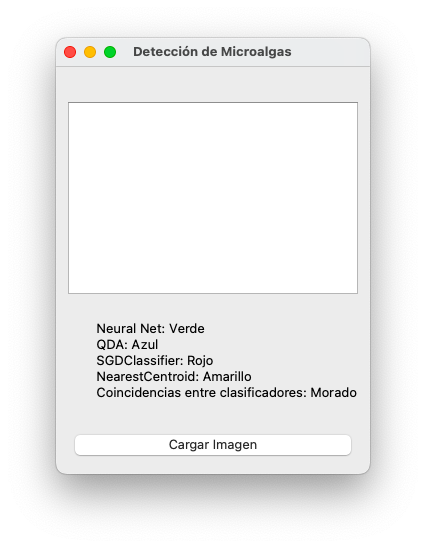
\includegraphics[width=.85\linewidth]{img/pantallaprincipal.png}}
    \caption{Interfaz al ejecutarse el programa}
    \label{fig:1}
\end{figure}

Para un primer caso de prueba, se utilizó una imagen que contiene 91 microalgas,  el sistema identificó posibles candidatos. En la figura \ref{fig:2} se muestra los candidatos identificados por el sistema.

\begin{figure}[h]
    \centering
    {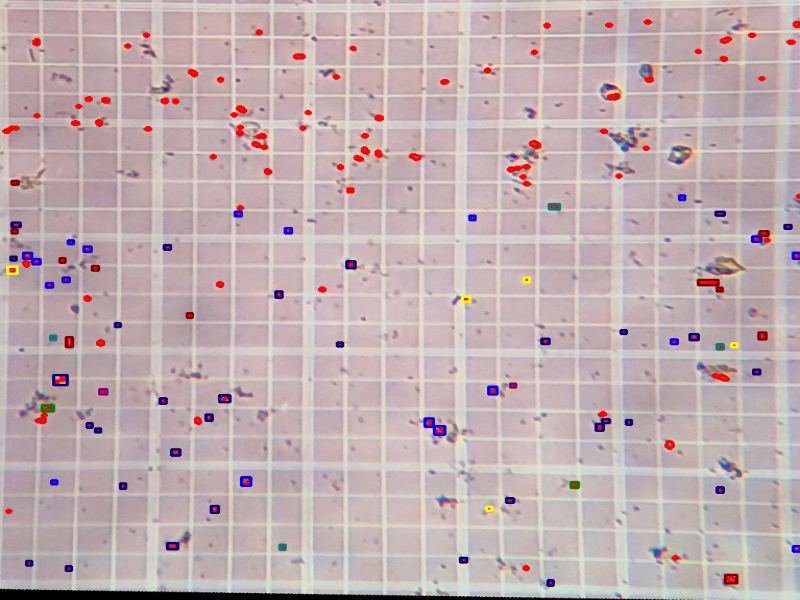
\includegraphics[width=.85\linewidth]{img/temp_processed_image10_1.png}}
    \caption{Posibles candidatos a microalgas identificados}
    \label{fig:2}
\end{figure}

\begin{figure}[h]
\centering
{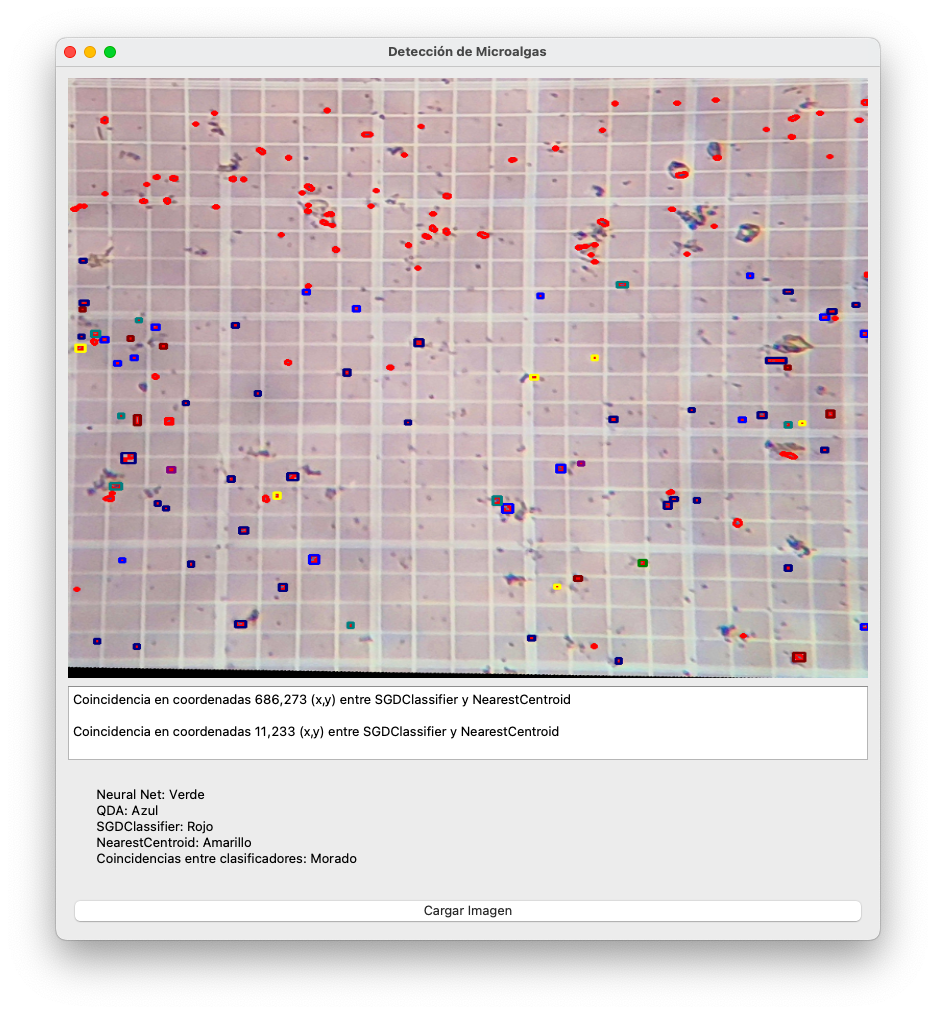
\includegraphics[width=.90\linewidth]{img/primerPrueba.png}}
\caption{Primera prueba de detección de microalgas }
\label{fig:3}
\end{figure}
Posteriormente, se enriqueció el dataset y se utilizaron 4 clasificadores para evaluar el procesamiento del modelo. Las microalgas consideradas son aquellas en las que al menos dos clasificadores coinciden en identificar la imagen como una microalga, como se puede observar en la figura \ref{fig:3}.

\begin{figure}[h]
\centering
{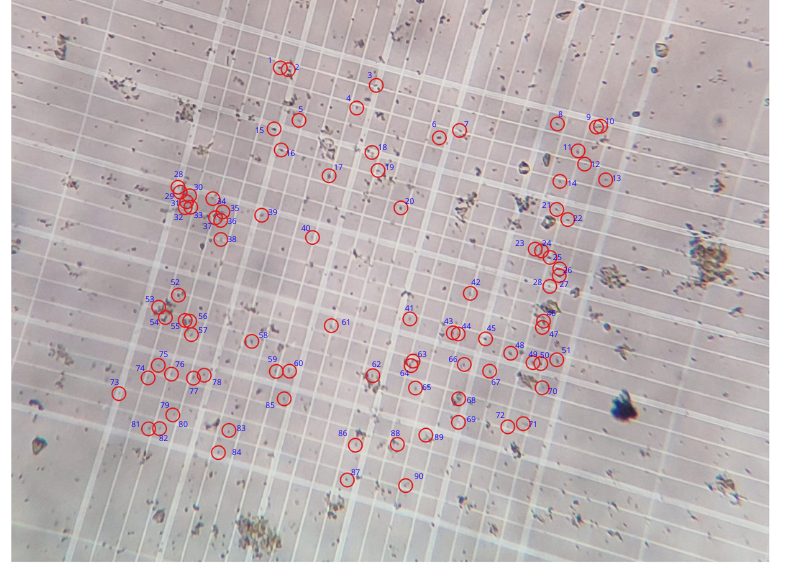
\includegraphics[width=.90\linewidth]{img/CONTEOMICROALGAS.png}}
\caption{Conteo de microalgas - Total 91 microalgas }
\label{fig:4}
\end{figure}

\subsection{Conteo de microalgas}

Al no  tener un número alto de asertividad de las pruebas se optó por hacer un análisis de los resultados obtenidos. El primer paso para realizar este análisis es hacer el etiquetado de la imagen para verificar el número de microalgas existentes en la imagen, dando como resultado un total de 91 microalgas, se puede observar en la figura \ref{fig:4}. También se estan tomando varios clasificadores para tener mayor precisión, cada clasificador tiene un color en especifico y se puede ver en la tabla \ref{TablaColorClasificador} en cual corresponde el color con su respectivo clasificador:
\begin{itemize}
    \item Neural Net
    \item  QDA
    \item SGDClassifier
    \item NearestCentroid
\end{itemize}
Al tener la combinación de estos podemos detectar mayor número de microalgas, considerando ls microalgas que detecta cada algoritmo y las que coinciden entre ellos. Para esto se colocaron diversos colores para identificar el clasificador que detectó dicha microalga y por su parte también un color en especifico por el match de clasificadores que coincidieron al detectar una microalga, a continuación la lista de colores que se utilizó para.

\begin{table}[h]
\centering
\begin{tabular}{|c|c|}
\hline
\textbf{Clasificador} & \textbf{Color} \\
\hline
Neural Net & \cellcolor[rgb]{0,1,0} Verde \\
\hline
QDA & \cellcolor[rgb]{0,0,1} Azul \\
\hline
SGDClassifier & \cellcolor[rgb]{1,0,0} Rojo \\
\hline
NearestCentroid & \cellcolor[rgb]{1,1,0} Amarillo \\
\hline
\end{tabular}
\caption{Tabla del color con su respectivo clasificador }
\label{TablaColorClasificador}
\end{table}

\begin{table}[h]
\centering
\begin{tabular}{|c|c|}
\hline
\textbf{Coincidencia} & \textbf{Color} \\
\hline
Neural Net \& QDA & \cellcolor[rgb]{0,0.5,0} Verde oscuro \\
\hline
Neural Net \& SGDClassifier & \cellcolor[rgb]{0.5,0,0.5} Morado \\
\hline
Neural Net \& NearestCentroid & \cellcolor[rgb]{0,0.5,0.5} Verde azulado oscuro \\
\hline
QDA \& SGDClassifier & \cellcolor[rgb]{0.5,0.5,0} Amarillo oscuro \\
\hline
QDA \& NearestCentroid & \cellcolor[rgb]{0,0,0.5} Azul oscuro \\
\hline
SGDClassifier \& NearestCentroid & \cellcolor[rgb]{0.5,0,0} Rojo oscuro \\
\hline
\end{tabular}
\caption{Tabla de coincidencia de los clasificadores }
\label{TablaConicidencia}
\end{table}

Las microalgas detectadas por uno y que tuvieron coincidencias entre los clasificadores son:
\begin{itemize}
    \item \textbf{Microalga 1:} Detectada por el clasificador SGDClassifier
    \item \textbf{Microalga 6:} Detectada por el clasificador SGDClassifier
    \item \textbf{Microalga 8:} Detectada por el clasificador SGDClassifier
    \item \textbf{Microalga 11:} Detectada por el clasificador SGDClassifier
    \item \textbf{Microalga 13:} Detectada por el clasificador SGDClassifier
    \item \textbf{Microalga 15:} Detectada por el clasificador SGDClassifier
    \item \textbf{Microalga 17:} Detectada por el clasificador SGDClassifier
    \item \textbf{Microalga 24:} Detectada por el clasificador QDA
    \item \textbf{Microalga 28:} Detectada por el clasificador QDA
    \item \textbf{Microalga 26:} Detectada por los clasificadores QDA y SGDClassifier
    \item \textbf{Microalga 32:} Detectada por los clasificadores Neural Net y NearestCentroid
    \item \textbf{Microalga 33:} Detectada por el clasificador QDA
    \item \textbf{Microalga 34:} Detectada por el clasificador QDA
    \item \textbf{Microalga 35:} Detectada por el clasificador QDA
    \item \textbf{Microalga 36:} Detectada por el clasificador QDA
    \item \textbf{Microalga 37:} Detectada por los clasificadores QDA y NearestCentroid
    \item \textbf{Microalga 40:} Detectada por los clasificadores QDA y NearestCentroid
    \item \textbf{Microalga 44:} Detectada por los clasificadores QDA y NearestCentroid
    \item \textbf{Microalga 46:} Detectada por los clasificadores QDA y NearestCentroid
    \item \textbf{Microalga 47:} Detectada por los clasificadores SGDClassifier y NearestCentroid
    \item \textbf{Microalga 48:} Detectada por los clasificadores SGDClassifier y NearestCentroid
    \item \textbf{Microalga 49:} Detectada por el clasificador QDA
    \item \textbf{Microalga 50:} Detectada por los clasificadores Neural Net y NearestCentroid 
    \item \textbf{Microalga 51:} Detectada por los clasificadores QDA y NearestCentroid 
    \item \textbf{Microalga 52:} Detectada por los clasificadores QDA y NearestCentroid
    \item \textbf{Microalga 53:} Detectada por los clasificadores QDA y NearestCentroid
    \item \textbf{Microalga 58:} Detectada por los clasificadores QDA y NearestCentroid
    \item \textbf{Microalga 59:} Detectada por el clasificador NearestCentroid
    \item \textbf{Microalga 64:} Detectada por los clasificadores Neural Net y SGDClassifier
    \item \textbf{Microalga 69:} Detectada por los clasificadores QDA y NearestCentroid
    \item \textbf{Microalga 71:} Detectada por los clasificadores QDA y NearestCentroid
    \item \textbf{Microalga 76:} Detectada por el clasificador QDA
    \item \textbf{Microalga 78:} Detectada por los clasificadores QDA y NearestCentroid
    \item \textbf{Microalga 82:} Detectada por los clasificadores QDA y NearestCentroid
    \item \textbf{Microalga 89:} Detectada por los clasificadores SGDClassifier y NearestCentroid
    \item \textbf{Microalga 90:} Detectada por los clasificadores Neural Net y NearestCentroid 
\end{itemize}

Las microalgas detectadas por los clasificadores individuales y por las coincidencias entre estos mismos se llegó a un resultado de 52 microalgas detectadas, dando un resultado medianamente favorable al detectar un poco más de la mitad de estas mismas. Se obtuvieron 23 falsos positivos, esto se tomo de las coincidencias entre dos clasificadores.

Para finalizar se realizó una matriz de confusión \ref{Tablaconfu} en la cual se explica el número de microalgas que si son y las que no son.


\begin{table}[t]
    \centering
    \begin{tabular}{ c | c | c | c | }
        \multicolumn{2}{c}{} & \multicolumn{2}{c}{} \\ \cline{3-4}
        \multicolumn{2}{c|}{} & Si & No  \\ \cline{2-4}
        \multirow{2}{*} & Si & 27 & 29\\ \cline{2-4}
        & No & 21 & 17 \\ \cline{2-4}
    \end{tabular}
    \caption{Tabla de confusión}
    \label{Tablaconfu}
\end{table}

\section{Conclusión}

En este trabajo se propone una solución al problema de reconocimiento de microalgas apartir de las imagenes proporcionadas, en la cual se le integró una interfaz grafica para mayor comodidad del usuario. Se creo un dataset para poder hacer uso de un clasificador y así entrenar a un modelo. Para lograrlo, se realizó una investigación sobre las distintas disitintas disciplinas, y se implementó en un programa con el lenguaje de programación Python.  El programa utiliza diversas librerías que llevan a la solución del problema como OpenCv y sklearn.

El proyecto desarrollado tenía como objetivo principal obtener significativamente un porcentaje de detección de microalgas favorable. Sin embargo, a pesar de los esfuerzos realizados, los resultados deseados no se lograron completamente debido a las limitaciones en la calidad y diversidad de las imágenes utilizadas para el entrenamiento del modelo. Es crucial que los conjuntos de datos de entrenamiento sean representativos y de alta calidad para garantizar una detección precisa. No obstante, para explorar y comparar diferentes enfoques de detección, se realizaron pruebas con cuatro clasificadores distintos: Neural Net, QDA, NearestCentroid y SGDClassifier.\\
La idea detrás de esta estrategia era evaluar el comportamiento y eficacia de cada clasificador en la tarea de detección de microalgas. Una característica interesante del sistema es que también verifica las coincidencias en las detecciones entre estos clasificadores, lo que puede proporcionar una mayor confianza en las detecciones acordadas por múltiples modelos. A través de esta metodología, se logró identificar un total de 52 microalgas a través de la concurrencia entre los cuatro modelos, lo que indica un potencial significativo en la combinación de múltiples técnicas de detección.

\addcontentsline{toc}{section}{Referencias} 
\printbibliography
%\balance



\end{document}

